%=============================================================================
% ..... THIS IS chapter{G.722: The ITU-T 64, 56, and 48 kbit/s wideband codec } .....
%  ... Revision:
% Oct.1995 - Created
% Jan.1996 - Peter Kroon revision
% Feb.2000 - Convergence towards STL2000
% Feb.2001 - Edits in example section
% Oct.2008 & august 2009 - Tool Update: introduction of G.192-compliant
%            bitstream basic operators and basic PLC options  -
%            Nicklas Sandgren, Jonas Svedberg, Balazs Kovesi, Adrien
%            Cormier, Claude Lamblin, Yusuke Hiwasaki
%=============================================================================
\chapter{G.722: The ITU-T 64, 56, and 48 kbit/s wideband
         speech coding algorithm}
%=============================================================================

With the emergence of ISDN networks offering digital connectivity at
64 kbit/s between subscribers, the possibility was given to improve
the standard telephone quality by increasing the transmitted
bandwidth. A bandwidth of 50-7000 Hz corresponding to a sampling of 16
kHz was chosen because it provides a substantial improvement of the
quality for applications where the speech is to be heard through
high quality loudspeakers e.g. for audio or video conference services,
commentary broadcasting, and high quality handsfree phones.

An expert group was created in November 1983 whose mandate was to
define a standard for 7 kHz speech coding within 64 kbit/s. After many
contributions received from several organisations, it has been decided
to choose a coder which combined subband filtering and adaptive
differential pulse-code modulation algorithms (SB-ADPCM). The final
recommendation was produced in March 1986 and approved in July 1986 by
the then CCITT SG XVIII as Recommendation ITU-T G.722 \cite{G.722}.

The full description on the implementation of the G.722 algorithm is
found in \cite{G.722}, and network aspects related to its operation
are found in \cite{G.725}. Figure \ref{fig:G.722-systemic} summarizes
some systemic aspects of the G.722 algorithm. Overview and notes on
the development of the G.722 algorithm can be found in several papers
\cite{G.722:General,G.722:Overview,G.722:SubjTest,G.722:Implementation,
 G.722:Modes,G.722:Applications}.  The following description of the
G.722 algorithm is based on the text in \cite{G.722:Summary}.

In 2006, upon ETSI DECT request, packet loss concealment (PLC)
procedures for G.722 were standardized to ensure a sufficient
robustness over the DECT wireless interface. ITU-T G.722 at 64 kbit/s
codec is the mandatory coder in ETSI New Generation DECT (NG-DECT)
standards (ETSI TS 102 527-1 and -3)
\cite{G.722:ETSITS102527-1,G.722:ETSITS102527-3}. These standards are
intended for wideband audio enabled devices to be connected on VoIP
networks.
 
In the above mentioned PLC standardization, G.722 software tool was
updated. Originally, the ITU-T G.722 algorithm used its own binary bit
stream format without synchronism headers; this made almost impossible
to apply frame errors. In the STL 2009, G.722 codec software tool was
made compliant with G.192 bitstream format and EID-XOR/G.192 style of
frame and bit error application to G.722 is enabled. At the same time,
STL basic operators and complexity counters were
introduced. Furthermore, the standalone decoder tool now includes
basic reference Packet Loss Concealment functionality.

%-----------------------------------------------------
%Box dimension: 19.16cm x 20.74cm
\begin{figure}[hbtp]
    \begin{center}
        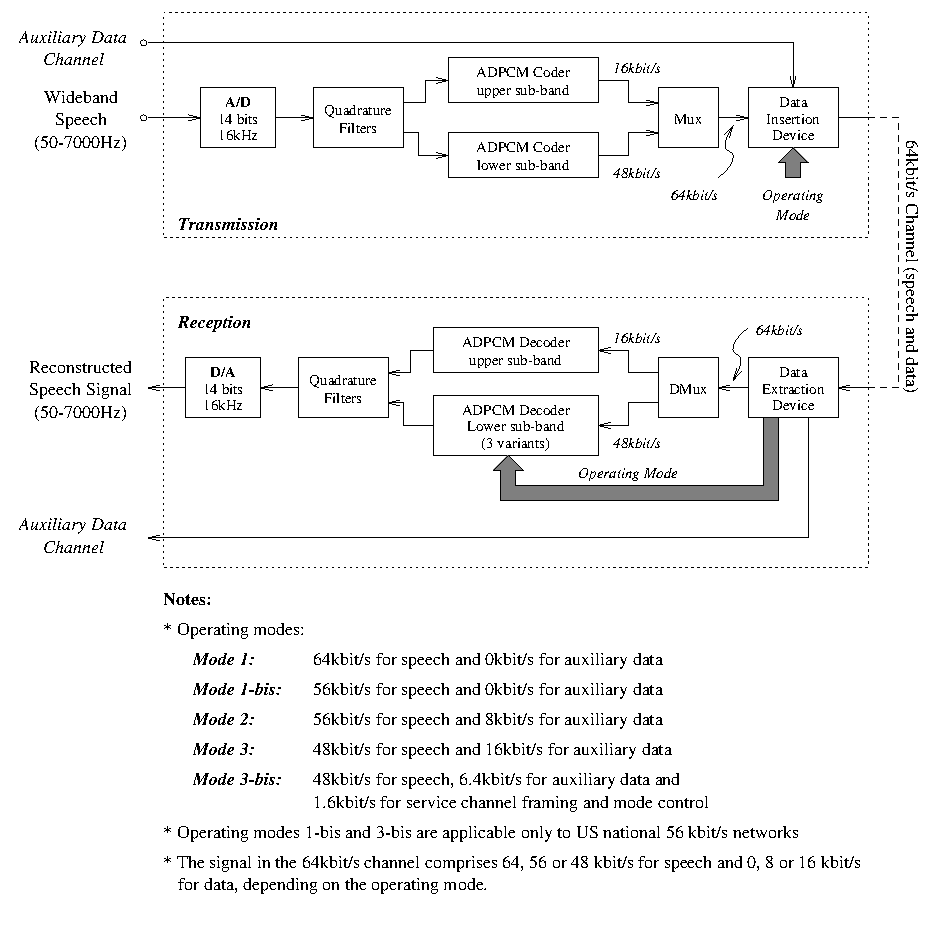
\includegraphics{g722}
  \end{center}
  \caption{G.722 encoder and decoder block diagrams
           \label{fig:G.722-systemic} }
\end{figure}
%-------------------------------------------------------------


%-----------------------------------------------------------------------------
\section{Description of the 64, 56, and 48 kbit/s G.722 algorithm}

In order to improve the transmitted speech quality, the input signal
has to be converted after antialiasing filtering by an
analog-to-digital (A/D) converter operating at 16 kHz sampling rate
and with a resolution of at least 14 uniform PCM bits. Similarly, at
the receive side, a digital-to-analog (D/A) converter operating at 16
kHz sampling rate and with a resolution of at least 14 uniform PCM
bits should be used. The specifications of the transmission
characteristics of the audio parts suited for the G.722 algorithm are
described in the Recommendation.  Some flexibility of the output bit
rate was implemented to allow the opening of an auxiliary data channel
within the 64 kbit/s channel.


%...............................................................
\subsection{Functional description of the SB-ADPCM encoder}\label{G722:descr-encoder}

Figure \ref{G722:encoder} shows block diagram of the SB-ADPCM encoder
which comprises the following main blocks.

%------------------------------
% G.722 Encoder
%------------------------------
\begin{figure}
    \begin{center}
    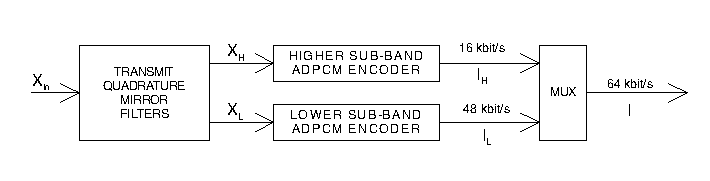
\includegraphics{g722-enc}
  \end{center}
  \caption{Block diagram of the SB-ADPCM encoder
           \label{G722:encoder}}
\end{figure}
%------------------------------

%-.-.-.-.-.-.-.-.-.-.-.-.-.-.-.-.-.-.-.-.-.-.-.-.-.-.-
\subsubsection{Transmit quadrature mirror filters}

The input signal $X_{in}$ is first filtered by two quadrature mirror
filters (QMF) which split the frequency band [0, 8000 Hz] into two equal
subbands. The outputs $X_{L}$ and $X_{H}$ of the lower and higher subbands are downsampled at 8 kHz by the filtering procedure.


%-.-.-.-.-.-.-.-.-.-.-.-.-.-.-.-.-.-.-.-.-.-.-.-.-.-.-
\subsubsection{Lower subband ADPCM encoder}

Figure \ref{G722:low-encoder} gives block diagram of the lower subband
ADPCM encoder. To transmit the lower band, the encoder was designed to
operate at 6, 5 or 4 bits per sample, corresponding to 48, 40 or 32
kbit/s, respectively. The ADPCM algorithm is very similar to the
embedded ADPCM algorithm of Recommendation ITU-T G.727
\cite{G.727}. It is an embedded ADPCM with 4 core bits and 2
additional bits. The embedded property was introduced to prevent
degradation in speech quality when the encoder and the decoder operate
during short intervals in different modes.

%------------------------------
% G.722 lower subband encoder
%------------------------------
\begin{figure}
    \begin{center}
    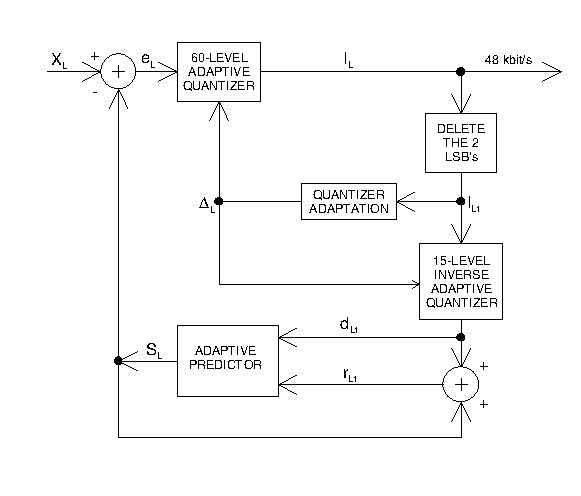
\includegraphics{g722-len}
  \end{center}
  \caption{Block diagram of the lower subband ADPCM encoder
           \label{G722:low-encoder}}
\end{figure}
%------------------------------

\paragraph{Adaptive quantizer}

A 60-level non-uniform adaptive quantizer is used to quantize the
difference $e_L$ between the input signal $X_{L}$ and the estimated
signal $S_{L}$. The output of the quantizer $I_{L}$ is the ADPCM
codeword for the lower subband. The 4 forbidden output codewords were
primarily introduced to prevent the generation of all zero codes at
all modes, but have also later been used to recover the 8 kHz content
used by the coder.


\paragraph{Inverse adaptive quantizer}

In the feedback loop the two least significant bits of $I_{L}$ are deleted to produce a 4 bit signal $I_{Lt}$ which is used for the adaptation of the quantizer scale factor and applied to a 15-level inverse adaptive quantizer to produce the quantized difference signal $d_{Lt}$.


\paragraph{Quantizer adaptation}

In order to maintain a wide dynamic range and minimize complexity, the
quantizer scale factor adaptation is performed in the base 2
logarithmic domain. The log-to-linear conversion is accomplished using
a lookup table. There is no adaptation of the speed control parameter
as in 32 kbit/s ADPCM \cite{G.726} because the encoder is designed to
transmit more than voiceband data.


\paragraph{Adaptive predictor and reconstructed signal computation}

The adaptive predictor structure is similar to the one used for G.727
ADPCM standard: 2 poles and 6 zeroes. The two sets of coefficients
(one for the poles and  the other for the zeroes section) are updated
using a simplified gradient algorithm. Stability constraints are
applied to the poles in order to prevent possible unstable
conditions. However, no predictor reset is applied for some specifics
inputs conditions as it is done in G.726 algorithm. The
reconstructed signal $r_{Lt}$ is computed by adding the quantized
difference signal $d_{Lt}$ to the signal estimate $S_{L}$ produced by the
adaptive predictor. The use of a 4-bit operation instead of a 6-bit
operation in the feedback loops of the lower band ADPCM encoder and
decoder allows for the insertion of data in the two least
significant bits without causing mistracking in the decoder.


%-.-.-.-.-.-.-.-.-.-.-.-.-.-.-.-.-.-.-.-.-.-.-.-.-.-.-
\subsubsection{Higher subband ADPCM encoder}

Figure \ref{G722:high-encoder} shows block diagram of the higher
subband ADPCM encoder. This encoder is designed to operate at 2 bits
per sample, corresponding to a fixed bitrate of 16 kbit/s. The
encoder algorithm is very similar to the lower band one but with the
following main differences. The quantizer is a 4-level non-linear
adaptive quantizer. The higher subband ADPCM encoder is not embedded,
hence the inverse quantizer uses the 2 bits in the feedback loop.

%------------------------------
% G.722 higher subband encoder
%------------------------------
\begin{figure}
    \begin{center}
    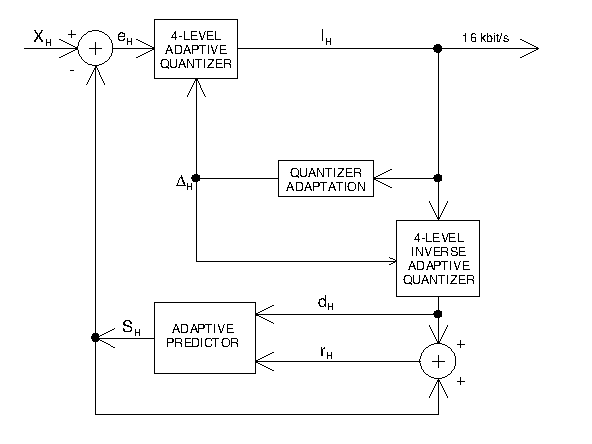
\includegraphics{g722-hen}
  \end{center}
  \caption{Block diagram of the higher subband ADPCM encoder
           \label{G722:high-encoder}}
\end{figure}
%------------------------------

%-.-.-.-.-.-.-.-.-.-.-.-.-.-.-.-.-.-.-.-.-.-.-.-.-.-.-
\subsubsection{Multiplexer}

The resulting codewords from the higher and lower subbands $I_H$ and
$I_L$ are combined to obtain the output codeword $I$ with an octet
format for transmission every 8 kHz frame resulting in 64~kbit/s. Note
that the 8 kHz clock may be provided by the network as it is always
done for 64 kbit/s A-law or $\mu$-law log-PCM (G.711) systems.


%...............................................................
\subsection{Functional description of the SB-ADPCM decoder}
            \label{G722:descr-decoder}

Figure \ref{G.722:decoder} shows block diagram of the SB-ADPCM decoder.


%-.-.-.-.-.-.-.-.-.-.-.-.-.-.-.-.-.-.-.-.-.-.-.-.-.-.-
\subsubsection{Demultiplexer}

The demultiplexer decomposes the received 64 kbit/s octet formatted
signal $I_r$ into two signals $I_{Lr}$ and $I_{Hr}$ which form the
codeword inputs for the lower and higher subband ADPCM decoders,
respectively.


%-.-.-.-.-.-.-.-.-.-.-.-.-.-.-.-.-.-.-.-.-.-.-.-.-.-.-
\subsubsection{Lower subband ADPCM decoder}

Figure \ref{G.722:low-decoder} shows a block diagram of the lower
subband decoder. This decoder operates in three different modes
depending on the received mode indication: 64, 56 and 48 kbit/s. The
block which produces the estimate signal is identical to the feedback
portion of the lower subband ADPCM encoder.  The reconstructed signal
$r_L$ is produced by adding the signal estimate to the relevant
quantized difference signals $d_{L,6}$, $d_{L,5}$ or $d_{L,4}$, which
are selected according to the received indication of the mode of
operation.


%-.-.-.-.-.-.-.-.-.-.-.-.-.-.-.-.-.-.-.-.-.-.-.-.-.-.-
\subsubsection{Higher subband ADPCM decoder}

This decoder (see Figure \ref{G.722:high-decoder}) is identical to the
feedback portion of the higher subband ADPCM encoder described in the
Section \ref{G722:descr-encoder}. Here, the output is reconstructed
signal $r_H$.

%------------------------------
% G.722 decoder
%------------------------------
\begin{figure}
    \begin{center}
        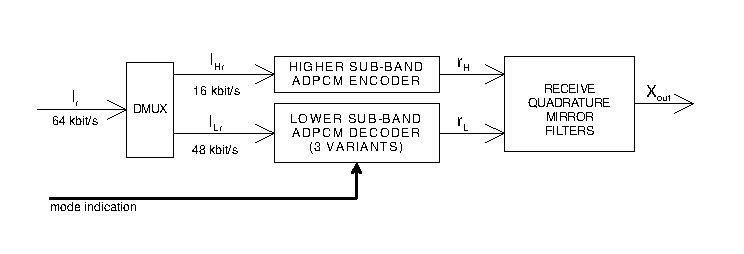
\includegraphics{g722-dec}
  \end{center}
  \caption{Block diagram of the SB-ADPCM decoder
           \label{G.722:decoder}}
\end{figure}
%------------------------------

%------------------------------
% G.722 lower subband decoder
%------------------------------
\begin{figure}
    \begin{center}
        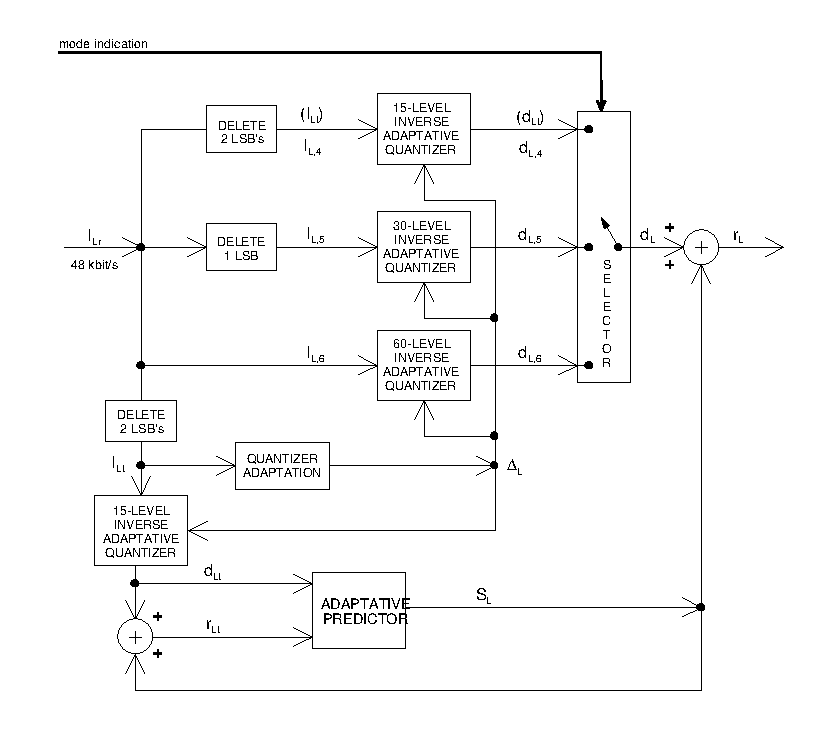
\includegraphics{g722-lde}
  \end{center}
  \caption{Block diagram of the lower subband ADPCM decoder
           \label{G.722:low-decoder}}
\end{figure}
%------------------------------

%------------------------------
% G.722 higher subband decoder
%------------------------------
\begin{figure}
    \begin{center}
        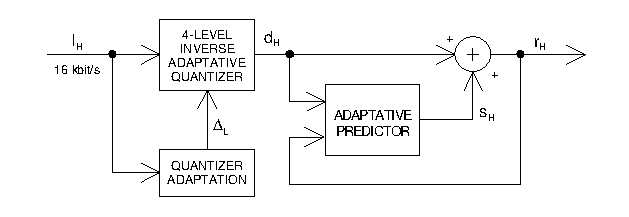
\includegraphics{g722-hde}
  \end{center}
  \caption{Block diagram of the higher subband ADPCM decoder
           \label{G.722:high-decoder}}
\end{figure}
%------------------------------

%-.-.-.-.-.-.-.-.-.-.-.-.-.-.-.-.-.-.-.-.-.-.-.-.-.-.-
\subsubsection{Receive QMF}

The receive QMF are two reconstruction filters which interpolate the
ouputs of the lower and higher subband ADPCM decoders from 8 to 16 kHz
($r_H$ and $r_L$) and generate 16~kHz sampling reconstructed output
$X_{out}$. Signal $X_{out}$ is converted to analog by the digital to
analog converter of the receiving side.

%...............................................................
\newpage

\subsection{Functional description of the basic Packet Loss Concealment functionality}

In 2006, basic index domain PLC functionality (zero index and frame
repeat algorithms) for detected frame errors were included in the
standalone decoder tool. The numbering and description of the four
basic algorithms provided can be seen in Table
\ref{tbl:G722StandaloneDecoder}.

\begin{table}[h]
  \begin{center}
  \begin{tabular}{|l|p{7cm}|}
	
\hline
PLC algorithm number & Description of concealment action \\
\hline
0 (default) & All bits in the erroneous frame are set to ``1''. (every 8 kHz octet index is set to 0xFF) \\
\hline
1	& same as PLC(0), but includes a decoder reset after the frame
decoding and synthesis operation.\\
\hline
2 & The bits from the previous frame(s) are repeated. After four erroneous frames, algorithm PLC(0) is used.  \\
\hline
3	& as PLC(2), but the first (0.625 ms) bits of the first good frame  after an erroneous frame are set to the value ``1''.  \\
\hline
  \end{tabular}
  \Caption{14cm}{\SF Basic PLC algorithms supported by the G.722 standalone decoder. \label{tbl:G722StandaloneDecoder}}
  \end{center}
\end{table}

The PLC actions in the G.722 standalone decoder are activated by
incoming G.192 frames that do not have a valid G192\_SYNC header
tag. Note that in November 2006, ITU-T SG16 approved two new
Appendices to G.722 for Packet Loss Concealment (PLC). These two
Appendices (Appendices III and IV \cite{G.722:AppIII,G.722:AppIV})
provide better quality over the basic PLC functionality included in
STL.

%-----------------------------------------------------------------------------
\section{Standalone G.192 compatible G.722 encoder and decoder tool}


\subsection{G.192 bit stream format for standalone G.722 encoder and decoder}

As described previously, G.722 is an embedded algorithm which supports
network scaling of the bitstream in three bitrates: 48, 56 and 64
kbit/s. To support this functionality within the G.192 file format the
G.722 encoder writes the 16 kbit/s embedded bits in the end of every
G.192 bitstream frame.
 
For every 16 kHz sample, there are eight G.722 encoded bits (an octet
index) to be transported in the G.192 frame. Bits b1 and b0 are the
embedded bits and bits b2-b7 are the non-embedded bits. In a G.192
frame, the b2 bits are written first in chunk, followed by that of b3,
until b7 bits. After all b7 bits are written, b1 bits are written and
then b0 bits. By sorting bits in this manner, truncation of a G.192
type G.722 frame bitstream from 64 kbit/s to 48 or 56 kbit/s is made
easy. Figures \ref{fig:G722trame}, \ref{fig:G722trame1} and
\ref{fig:G722trame2} show how the G.192 frames are composed for
various bit rates (64, 56, 48 kbit/s) and example frame sizes (10, 5,
20 ms). G.192 format is useful for enhanced simulation of G.722,
however actual application transport formats may be different (e.g. as
defined in \cite{G.722} and as used in \cite{G.722:RFC3551}).

\begin{figure}[h]
    \begin{center}
        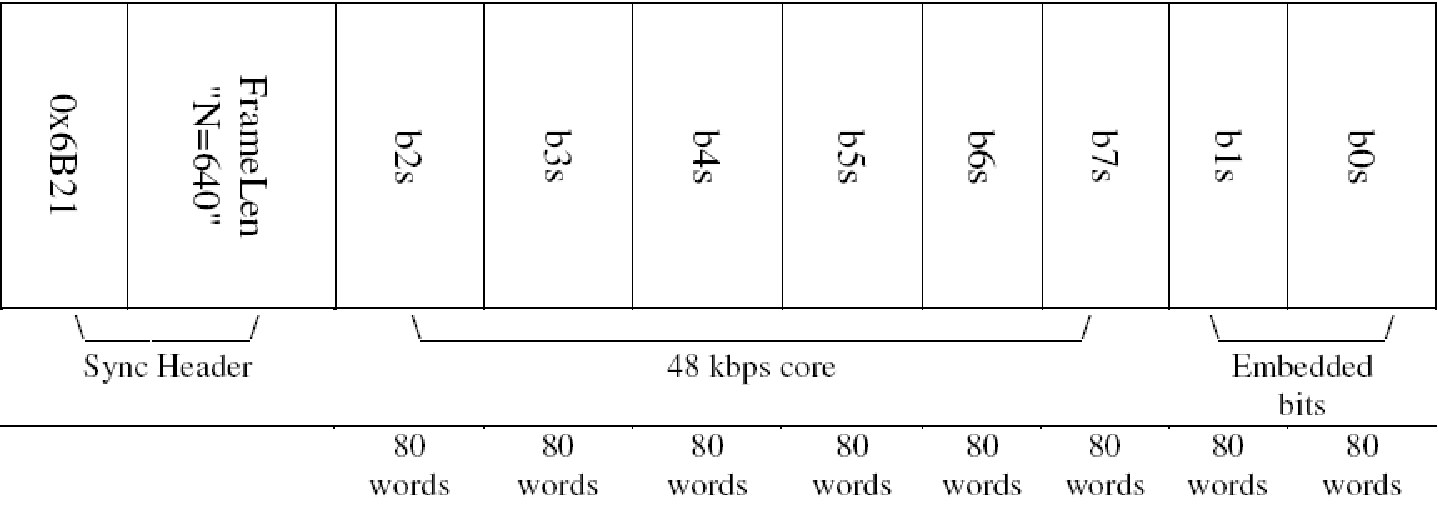
\includegraphics[scale=0.5]{G722trame}
  \end{center}
  \caption{Example of a G.192 compatible G.722 encoder output frame for a 10 ms input frame size. This frame has a length of 640 bits and a G192\_SYNC (0x6B21) header tag, in the G.192 file each g722 bit is stored as a 16 bit word.
           \label{fig:G722trame}}
\end{figure}

\pagebreak 

\begin{figure}[hbt]
    \begin{center}
      % 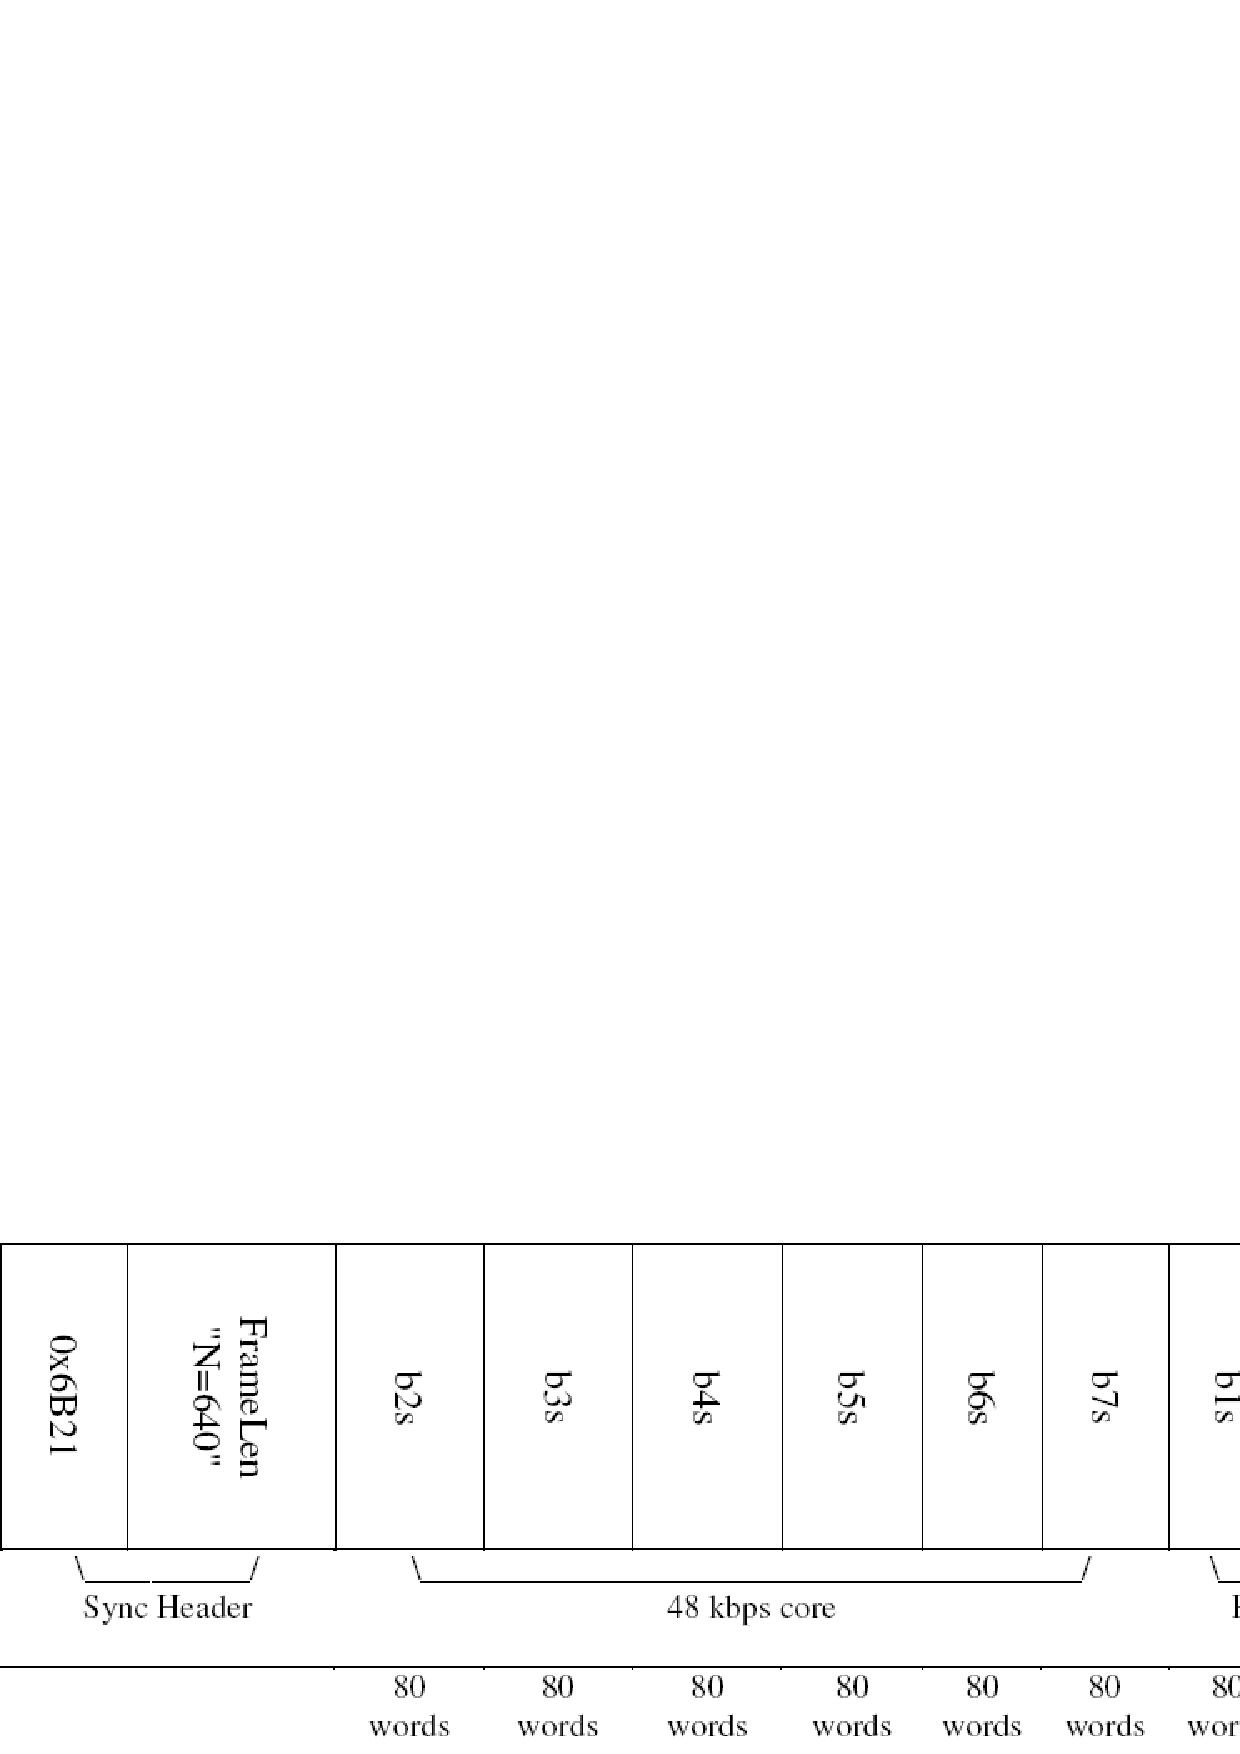
\includegraphics[scale=0.5]{G722trame1}
        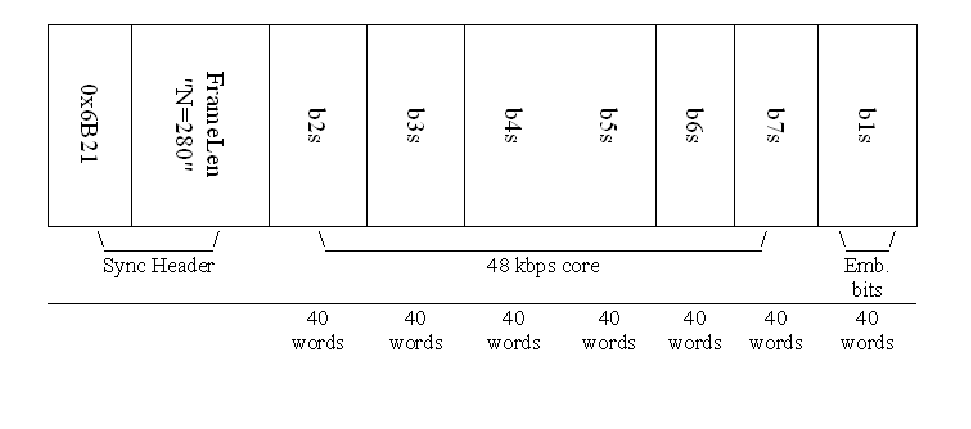
\includegraphics[scale=0.8]{G722trame1new}
%        \includegraphics[scale=0.5]{figure_g722_5ms_280bits.ps}
	    \caption{ Example of a G.192 compatible G.722 56 kbit/s encoder output frame for a 5 ms input frame size. This frame						has a length of 280 bits and a G192\_SYNC (0x6B21) header tag.
        \label{fig:G722trame1}}
	 \end{center}
\end{figure}

\begin{figure}[h]
    \begin{center}
        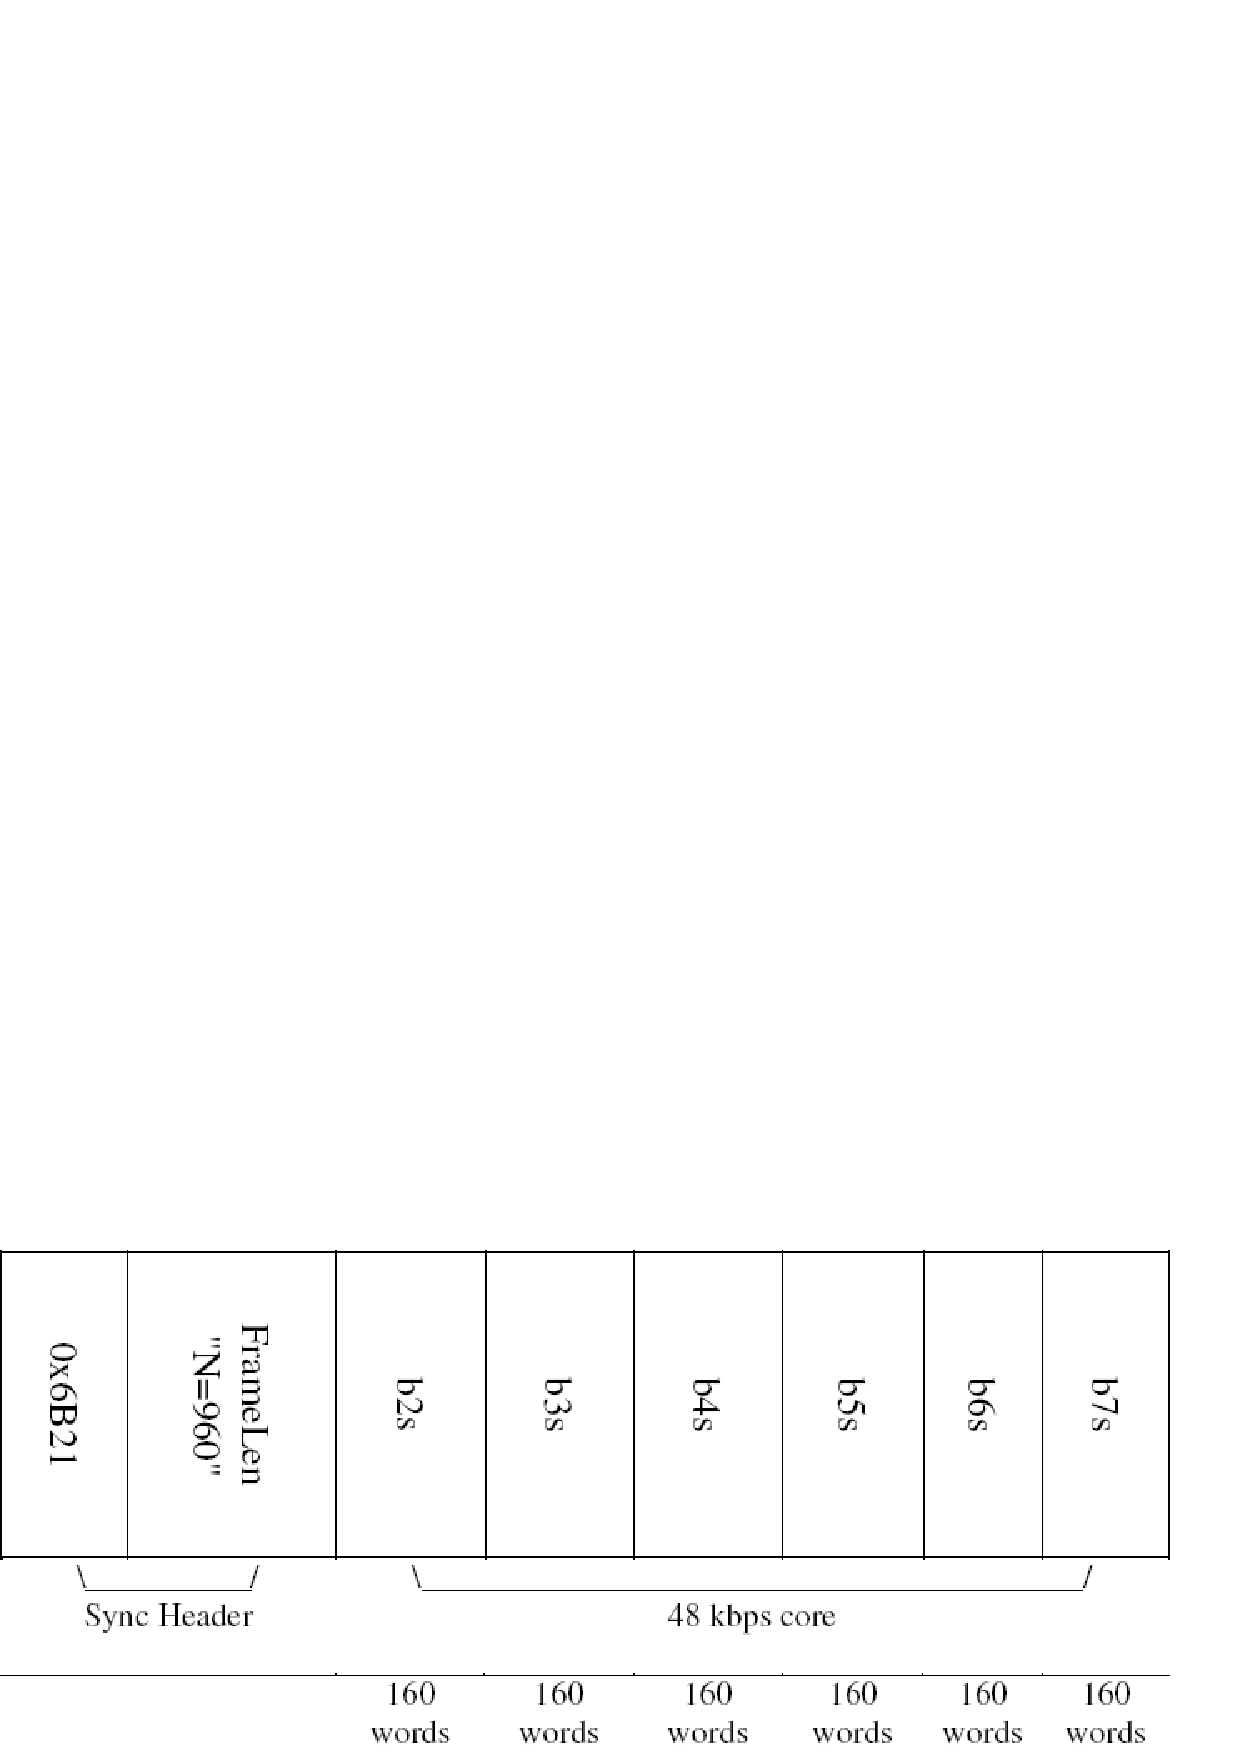
\includegraphics[scale=0.5]{G722trame2}
  \end{center}
  \caption{Example of G.192 compatible G.722 48 kbit/s encoder output frame for a 20 ms input frame size. This frame has a length of 960 bits and a G192\_SYNC (0x6B21) header tag.
           \label{fig:G722trame2}}
\end{figure}

\subsection{Standalone G.722 Encoder specific operation}

If the encoder can not read a complete input frame it stops its processing, this means that the final decoder output file may be up to a frame shorter than the input speech file. 

\pagebreak 

%-----------------------------------------------------------------------------
\section{ITU-T STL G.722 Implementation}

This implementation of the G.722 algorithm is composed of several
source files. The interface routines are in file {\tt g722.c}, with
prototypes in {\tt g722.h}. The original code of the STL G.722 was
provided by CNET/France and its user interface was modified to be
consistent with the other software modules of the STL. The update to
make G.722 tool compliant with G.192 bit stream format and include
basic PLC functionality was performed by Ericsson. The basic operators
and complexity counters were introduced by France Telecom.

The problem of storing the state variables was solved by defining a
structure called {\tt g722\_state} which containing all the necessary
state variables.  By means of this approach, several streams may be
processed in parallel\footnote{\SF This feature was not possible with
the original code provided by CNET and was added in the modifications
of the user interface.}, provided that one structure is assigned (and
that one call to the encoding/decoding routines is done) for each
data stream (this can be advantageous for machines with support for
parallel processing). The G.722 state structure has the following
fields (which are all {\tt shorts}):

\rulex{1pt} \hfill \begin{minipage}{150mm} \normalsize
 {\em ah, al} \hfill \pbox{120mm}{Second-order pole section coefficient
        buffer for higher and lower band, respectively}\\*[1mm]
 {\em bh, bl} \hfill \pbox{120mm}{Seventh-order zero section coefficient
        buffer for higher and lower band, respectively}\\*[1mm]
 {\em deth, detl} \hfill \pbox{120mm}{Delayed quantizer scale factor
        for higher and lower band, respectively}\\*[1mm]
 {\em dh} \hfill \pbox{120mm}{Quantizer difference signal memory}\\*[1mm]
 {\em dlt} \hfill \pbox{120mm}{Quantizer difference signal for the adaptive
        predictor}\\*[1mm]
 {\em init\_qmf\_rx} \hfill \pbox{120mm}{Flag indicating the need to
        initialize the QMF filters on the reception (decoder) side}\\*[1mm]
 {\em init\_qmf\_tx} \hfill \pbox{120mm}{Flag indicating the need to
        initialize the QMF filters on the transmission (encoder) side}\\*[1mm]
 {\em nbh, nbl} \hfill \pbox{120mm}{Delayed logarithmic quantizer factor
        for higher and lower band, respectively}\\*[1mm]
 {\em ph, plt} \hfill \pbox{120mm}{Partially reconstructed signal memory
        for higher and lower band, respectively}\\*[1mm]
 {\em qmf\_rx\_delayx} \hfill \pbox{120mm}{Memory of past 24 received (decoded)
        samples}\\*[1mm]
 {\em qmf\_tx\_delayx} \hfill \pbox{120mm}{Memory of past 24 transmitted
        (encoded) samples}\\*[1mm]
 {\em rh[3]} \hfill \pbox{120mm}{Quantized reconstructed signal}\\*[1mm]
 {\em rlt[3]} \hfill \pbox{120mm}{Reconstructed signal memory for the
        adaptive predictor}\\*[1mm]
 {\em sh, sl} \hfill \pbox{120mm}{Predictor output value for higher
        and lower band, respectively}\\*[1mm]
 {\em sph, spl} \hfill \pbox{120mm}{Pole section output signal for higher
        and lower band, respectively}\\*[1mm]
 {\em szh, szl} \hfill \pbox{120mm}{Zero section output signal for higher
        and lower band, respectively}\\
\end{minipage}

The default bitstream generated by the STL G.722 encoder is a G.192
compatible 16 bit output file and it is provided using the frame size
specified by the -fsize command. Bits in a G.192 bitstream frame are
ordered so that the frame can be truncated at 56 and 48 kbit/s. If the
number of input samples are non divisible by the frame size, the
output codeword stream is truncated at the last frame boundary.

A legacy g722 octet stream can be obtained using the option -byte.
The legacy bitstream generated by the STL G.722 encoder has 8 valid
bits for each encoded sample, saved in right-justified
{\short}s. i.e., the codewords are located in the lower 8-bits of the
encoded bitstream file. The MSB is always 0 for the 16 bit bitstream
file. The lower 6 bits are the lower-subband encoded bits, and the
upper two bits of the 8 valid bits are the upper-subband encoded
bits. When the decoder is not in operation mode 1, the decoder will
discard 1 or 2 of the lower bits of the lower-subband. It should be
noted that, when bit errors are inserted in this bitstream and the
operation mode is not mode 1, the actual bit error rate seen by the
decoder may not be the one actually desired. One may consider that, in
simulating a system where auxiliary data channels are used, such as
modes 2 and 3, this is actually the desired behaviour, because errors
hitting the auxiliary data will not affect the decoded speech
quality. However, if simulation of modes 1-bis or 3-bis is intended,
then the some of the errors hitting the lower 1 (mode 1-bis) or 2 bits
(mode 3-bis) will not be seen by the decoder, and the overall bit
error rate will actually be smaller than the desired one. There are
two possible approaches to circumvent this problem:
\begin{itemize}
 \item  the use of an external program to shift the bitstream samples
   one or two bits (respectively for modes 1-bis or 3-bis) to the right
   before the bitstream serialization process for use with the STL EID
   module, and an external program to left-shift
   the bitream samples by one or two bits after error insertion and
   before using the STL G.722 decoder. This solution is valid for both
   random and burst bit errors.
 \item  to increase proportionally the bit error rate by 1/8 (mode 1-bis) or
   1/4 (mode 3-bis), to statistically compensate for errors hitting unused 
   bits. This solution is valid only for random bit errors.
\end{itemize}

From the users' perspective, the encoding function is {\tt
g722\_encode}, and the decoding function is {\tt g722\_decode}.
Before using these functions, state variables for the encoder and the
decoder must be initialized respectively by {\tt g722\_reset\_encoder}
and {\tt g722\_reset\_decoder}. It should be noted that encoder and
decoder need individual state variables to work properly.

In the following part a summary of calls to the three entry functions
is found.

\subsection{{\tt g722\_encode}}

{\bf Syntax: }

{\tt
\#include "g722.h"\\
long g722\_encode (\ttpbox{110mm}{
            short {\em *inp\_buf},
            short {\em *g722\_frame},
            long  {\em smpno},
            g722\_state {\em *g722\_encode});
         }
}

{\bf Prototype: }    g722.h

{\bf Description: }

        Simulation of the ITU-T G.722 64 kbit/s encoder. Takes
        the linear (16-bit, left-justified) input array
        of shorts {\em inp\_buf} (16 bit,
        right-justified, without sign extension) with {\em smpno}
        samples, and saves the encoded bit-stream in the array of shorts
        {\em g722\_frame}. 

        The state variables are saved in the structure pointed by {\em
        g722\_encode}, and the reset can be established by making a
        call to {\tt g722\_reset\_encoder}.

{\bf Variables: }
\begin{Descr}{\DescrLen}
\item[\pbox{20mm}{\em inp\_buf}] %\rulex{1mm}\\
               Is the input samples' buffer with {\em smpno}
               left-justified 16-bit linear {\tt short} speech samples.

\item[\pbox{20mm}{\em g722\_frame}] %\rulex{1mm}\\
               Is the encoded samples' buffer; each {\tt short} sample
               will contain the encoded parameters as right-justified
               8-bit samples.

\item[\pbox{20mm}{\em smpno}] %\rulex{1mm}\\
               Is a long with the number of samples to be encoded from
               the input buffer {\em inp\_buf}.

\item[\pbox{20mm}{\em g722\_encode}] %\rulex{1mm}\\
               A pointer to the state variable structure; all the variables
               here are for
               internal use of the G.722 algorithm, and should not be
               changed by the user. Fields of this structure are described
               above.
\end{Descr}

        {\bf Return value: }

Returns the number of speech samples encoded.


\newpage
\subsection{{\tt g722\_decode}}

{\bf Syntax: }

{\tt
\#include "g722.h"\\
short g722\_decode (\ttpbox{110mm}{
            short {\em *g722\_frame},
            short {\em *out\_buf},
            int  {\em mode},
            long  {\em smpno},
            g722\_state {\em *g722\_decoder}, );
         }
}

{\bf Prototype: }    g722.h

\enlargethispage*{12mm}
{\bf Description: }

        Simulation of the ITU-T 64 kbit/s G.722 decoder. Reconstructs
        a linear (16-bit, left-justified) array
        of shorts {\em inp\_buf} (16 bit,
        right-justified, without sign extension) with {\em smpno}
        samples from the encoded bit-stream in the array of shorts
        {\em g722\_frame}. Include a basic Packet Loss Concealment functionality.

        The state variables are saved in the structure pointed by {\em
        g722\_decoder}, and the reset can be established by making a
        call to {\em g722\_reset\_decoder}.

{\bf Variables: }
\begin{Descr}{\DescrLen}
\item[\pbox{20mm}{\em g722\_frame}] %\rulex{1mm}\\
               Is the encoded samples' buffer; each {\tt short} sample
               will contain the encoded parameters as right-justified
               8-bit samples.

\item[\pbox{20mm}{\em out\_buf}] %\rulex{1mm}\\
               Is the output samples' buffer with {\em smpno}
               left-justified 16-bit linear {\tt short} speech samples.

\item[\pbox{20mm}{\em mode}] %\rulex{1mm}\\
               Is an {\tt int} which indicates the operation mode for the
               G.722 decoder. If equal to 1, the decoder will operate at
               64 kbit/s. If equal to 2, the decoder will operate at
               56 kbit/s, discarding the least significant bit of the
               lower-band ADPCM. If equal to 3, the decoder will
               discard the two least significant bits of the lower
               band ADPCM, being equivalent to the 48 kbit/s operation of
               the G.722 algorithm. It should be noted that, for this
               implementation of the G.722 algorithm, mode 1-bis is
               identical to mode 2, and mode 3-bis is identical to mode 3.

\item[\pbox{20mm}{\em smpno}] %\rulex{1mm}\\
               Is a long with the number of samples in the input
               encoded sample buffer {\em g722\_frame} to be decoded.

\item[\pbox{20mm}{\em g722\_decoder}] %\rulex{1mm}\\
               A pointer to the state variable structure; all the variables
               here are for
               internal use of the G.722 algorithm, and should not be
               changed by the user. Fields of this structure are described
               above.
\end{Descr}

        {\bf Return value: }

Returns the number of speech samples encoded.


\newpage
\subsection{{\tt g722\_reset\_encoder}}

{\bf Syntax: }

{\tt
\#include "g722.h"\\
     void g722\_reset\_encoder (g722\_state {\em *g722\_encoder});
}

{\bf Prototype: }    g722.h

{\bf Description: }

        Initializes the state variables for the G.722 encoder or decoder.
        Coder and decoder require each a different state variable.

{\bf Variables: }
\begin{Descr}{\DescrLen}
\item[\pbox{20mm}{\em g722\_encoder}] %\rulex{1mm}\\
        A pointer to the G.722 encoder state variable structure which
        is to be initialized.
\end{Descr}

{\bf Return value: }    None.


\subsection{{\tt g722\_reset\_decoder}}

{\bf Syntax: }

{\tt
\#include "g722.h"\\
  void g722\_reset\_decoder (g722\_state {\em *g722\_decoder});
}

{\bf Prototype: }    g722.h

{\bf Description: }

        Initializes the state variables for the G.722 decoder.
        Coder and decoder require each a different state variable.

{\bf Variables: }
\begin{Descr}{\DescrLen}
\item[\pbox{20mm}{\em g722\_decoder}] %\rulex{1mm}\\
        A pointer to the G.722 decoder state variable structure which
        is to be initialized.
\end{Descr}


{\bf Return value: }       None.

\newpage

%-----------------------------------------------------------------------------
\section{Portability and compliance}

The portability test for these routines has been performed using the
test sequences designed by the ITU-T for the G.722 algorithm\footnote{
  The G.722 test sequences are freely downloadable from
  http://www.itu.int/rec/T-REC-G.722-198703-I!AppII/en.}. It should be
noted that the G.722 test sequences are not designed to test the QMF
filters, but only to exercise the upper and lower band encoder and
decoder ADPCM algorithms. Therefore, testing of the codec with the
test sequences was done with a special set of test programs that used
the core G.722 upper- and lower-band ADPCM coding and decoding
functions. All test sequences were correctly processed.

This module has been compiled and tested on PC platform with Cygwin (CYGWIN\_NT-5.0), using gcc(3.3.3), and with Microsoft Visual Studio 8. 

Please note that the 16 bit oriented G.192 files require correct octet
swapping of inputs and outputs on big/little-endian machines.

%-----------------------------------------------------------------------------
\section{Encoder(encg722) tool command line options}

{\tt\small
\begin{verbatim}

Usage:
encg722  [-options] InpFile OutFile  
where:
InpFile     is the name of the speech file to be processed;
OutFile     is the name with the processed bitstream;

options:
-fsize  #   Number of 16 kHz input samples per frame (must be an even number).
            Default is 160 samples (16 kHz) (10 ms)  
-mode   #   Operating mode (1,2,3) (or rate 64, 56, 48 in kbit/s). 
            Default is mode 1 (= 64 kbit/s)
-frames #   number of frames to process
            (values -1 or 0 processes the whole file )
-byte       Provide encoder output data in legacy octet format.
            (default is g192). 			   
-h/-help    print help message


\end{verbatim}
}

%-----------------------------------------------------------------------------
\section{Decoder (decg722) tool command line options}
{\tt\small
\begin{verbatim}
Usage:

decg722 [-options] InpFile OutFile

where:
InpFile     is the name of the bit stream input file;
OutFile     is the name of the file with synthesized speech;

options:

-mode #     is the operation mode for the G.722 decoder.
            Default is mode 1/64 kbit/s.
            (others are mode 2/56 kbit/s and mode 3/48 kbit/s)

-fsize #    Number of samples per frame  
            Default is 160, 16 kHz samples (or 10ms)
            (NB! must be the same as on the encoder side.) 

-frames #   Number of frames to process

-plc #      Packet Loss Concealment algorithm number
            (0 = zero index insertion, no decoder state reset)
            (1 = zero index insertion, decoder state reset)
            (2 = previous frame repetition, no decoder state reset)
            (3 = previous frame repetition, a few zero_indeces in first good
             frame, no decoder state reset)
  
-byte       Use legacy nonG192 G.722 format (byte oriented) without
            frame/synch headers.

-h/-help    print help message
\end{verbatim}
}

%-----------------------------------------------------------------------------
\section{Example code}

%..........................................................................
\subsection {Description of the demonstration programs}

One demonstration program is provided for the G.722 module,
g722demo.c. In addition, two programs are provided in the distribution
when compliance testing of the encoder and decoder is necessary,
tstcg722.c and tstdg722.c\footnote{\SF. The demonstration program g722demo.c cannot be used for compliance verification because the test vectors for G.722 do not foresee processing through the quadrature mirror
filters.}. 

Program {\tt g722demo.c} accepts 16-bit, linear PCM samples sampled at
16 kHz as encoder input. The decoder also produces files in the same
format. The bitstream signals out of the encoder are always organized
in 16-bit, right-justified words that use the lower 8 bits (i.e., 64
kbit/s). According to the user-specified mode, the decoder will decode
the G.722-encoded bitstream using 64, 56, or 48 kbit/s (i.e. full 8
bits, discard 1 bit of the lower band, or discard 2 bits of the lower
band). 
It should be noted that the demonstration programs g722demo.c, tstcg722.c and tstdg722.c only produce G.722 legacy bitstream. To produce bitstream compliant with G.192, please use encg722.c and decg722.c. Similarly, basic PLC functionnality is not supported the demonstration programs g722demo.cand tstdg722.c. Please use decg722.c for basic PLC functionnality.

%..........................................................................
\subsection {Simple example}

The following C code gives an example of G.722 coding and decoding
using as input wideband speech which is encoded and decoded at either
64, 56, or 48 kbit/s, according to the user-specified parameter
{\em mode}.
{\tt\small
\begin{verbatim}
#include <stdio.h>
#include "ugstdemo.h"
#include "g722.h"
#define BLK_LEN 256

void main(argc, argv)
  int             argc;
  char           *argv[];
{
  g722_state      encoder_state, decoder_state;
  int             mode;
  char            FileIn[180], FileOut[180];
  short           smpno, tmp_buf[BLK_LEN], inp_buf[BLK_LEN], out_buf[BLK_LEN];
  FILE           *Fi, *Fo;

  /* Get parameters for processing */
  GET_PAR_S(1, "_Input File: .................. ", FileIn);
  GET_PAR_S(2, "_Output File: ................. ", FileOut);
  GET_PAR_I(3, "_Mode: ........................ ", mode);

  /* Initialize state structures */
  g722_reset_encoder(&encoder_state);
  g722_reset_decoder(&decoder_state);

  /* Opening input and output 16-bit linear PCM speech files */
  Fi = fopen(FileIn, RB);
  Fo = fopen(FileOut, WB);

 /* File processing */
  while (fread(inp_buf, BLK_LEN, sizeof(short), Fi) == BLK_LEN)
  {
    /* Encode input samples in blocks of length BLK_LEN */
    smpno = g722_encode(inp_buf, tmp_buf, BLK_LEN, &encoder_state);

    /* Decode G.722-coded samples in blocks of length BLK_LEN */
    smpno = g722_decode(tmp_buf, out_buf, mode, smpno, &decoder_state);

    /* Write 16-bit linear PCM output decoded samples */
    fwrite(out_buf, smpno, sizeof(short), Fo);
  }

  /* Close input and output files */
  fclose(Fi); fclose(Fo);
}
\end{verbatim}
}

%..........................................................................
\subsection {Example operation of encoder (encg722)}
{\tt\small
\begin{verbatim}
foreach mode ( 1 2 3 ) # (corresponds to 64,56,48 kbit/s)
   foreach fsize ( 160 320 640) # (corresponds to 10,20,40 ms) 
      encg722  -mode $mode -fsize $fsize inpsp.smp outp.g722.$fsize.$mode.g192 
   end #fsize 
end #mode
\end{verbatim}
}

%..........................................................................
\subsection {Example operation of decoder (decg722)}
{\tt\small
\begin{verbatim}
foreach mode ( 1 2 3 ) # (corresponds to 64,56,48 kbit/s)
   foreach fsize ( 160 320 640) # (corresponds to 10,20,40 ms) 
      decg722 -plc 0 -fsize $fsize outp.g722.$fsize.$mode.g192  outsp.smp
      mv outpsp.smp outpsp.g722.$fsize.$mode.plc.0.smp 
   end #fsize
end #mode
\end{verbatim}
}
